\documentclass[../talk.tex]{subfiles}
\begin{document}


    	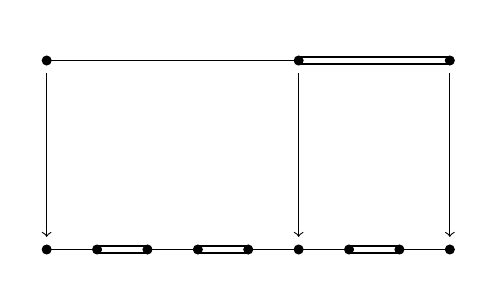
\begin{tikzpicture}[scale=.8]
    		\newcommand{\orig}{-1.5}
    		\newcommand{\trans}{.8}
    		\newcommand{\vertspac}{-3.}
    		\newcommand{\del}{.2}
    		\newcommand{\rad}{2pt} % radii of the circles
    	
    		% set the style of the strong bonds
    		\tikzset{
    			strong/.style={
    				double,
    				double distance=\rad,
    				line width=0.5pt
    				}
    		}
    		
    		% initial chain
    	
    		% bonds 
        	\draw[-] (\orig, \vertspac)  node [left] {}  -- (\orig+\trans, \vertspac);%  node [midway, above] {$t_w$};
			\draw[strong] (\orig+\trans,\vertspac) -- (\orig+2*\trans,\vertspac);%  node [midway, above] {$t_s$};
			\draw[-] (\orig+2*\trans,\vertspac) -- (\orig+3*\trans,\vertspac);% node [midway, above] {$t_w$};	
			\draw[strong] (\orig+3*\trans,\vertspac) -- (\orig+4*\trans,\vertspac);% node [midway, above] {$t_s$};
			\draw[-] (\orig+4*\trans,\vertspac) -- (\orig+5*\trans,\vertspac);% node [midway, above] {$t_w$};
			\draw[-] (\orig+5*\trans,\vertspac) -- (\orig+6*\trans,\vertspac);% node [midway, above] {$t_w$};
			\draw[strong] (\orig+6*\trans,\vertspac) -- (\orig+7*\trans,\vertspac);% node [midway, above] {$t_s$};
			\draw[-] (\orig+7*\trans,\vertspac) -- (\orig+8*\trans,\vertspac);% node [midway, above] {$t_w$};
    	
    		% sites
			\foreach \x in {0,...,8}
		      \filldraw (\orig+\x*\trans,\vertspac) circle (\rad); % node [below] {$\ket{\x}$};
		      
		    \filldraw (\orig+5*\trans,0) circle (0) node [shift={(-0.4,0.3)}] {};
		    
		    % vertical arrows
		    \draw [->] (\orig,-\del) -- (\orig,\vertspac+\del) node [midway, right] {};
		    \draw [->] (\orig+5*\trans,-\del) -- (\orig+5*\trans,\vertspac+\del) node [midway, right] {};
		    \draw [->] (\orig+8*\trans,-\del) -- (\orig+8*\trans,\vertspac+\del) node [midway, right] {};
		      
		    % atomic chain
		    
        	\draw[-] (\orig, 0*\vertspac)  node [left] {}  -- (\orig+5*\trans, 0*\vertspac);%  node [midway, above] {$t_w'$};
			\draw[strong] (\orig+5*\trans,0*\vertspac) -- (\orig+8*\trans,0*\vertspac);% node [midway, above] {$t_s'$};
			
			\filldraw (\orig,0*\vertspac) circle (\rad); % node [below] {$\ket{\x}$};
			\filldraw (\orig+5*\trans,0*\vertspac) circle (\rad) node [shift={(-0.7,0.3)}] {};
			\filldraw (\orig+8*\trans,0*\vertspac) circle (\rad)node [right] {};
		\end{tikzpicture}

\end{document}